% Chapter 3

\chapter{Key Concepts and Terms About Cyber newsfeed} % Main chapter title

\label{Chapter3key_concepts-and-terms} % For referencing the chapter elsewhere, use \ref{Chapter3} 

%----------------------------------------------------------------------------------------



%----------------------------------------------------------------------------------------

\section{Introduction} 
This chapter provides key concepts, 
keywords and important terms which are both 
1) about the cyber newsfeeds and 
2) are related to cyber newsfeeds.
I have used the mindmap approach \citep{buzan2006mind}  
to list the central concepts first 
and then map the required concepts 
in relation to each other\footnote{Refer to Appendix \ref{AppendixChapter3} for more details}. 
Understanding the concepts mentioned in the mindmap 
are required to understand the problem context 
and the subsequent chapters of this master thesis. 
The terms and the concepts introduced in this chapter 
are relevant throughout the rest of this master thesis. I have made use of tools, technology, prototype and artefact for \enquote{Cybernewsfeed Technology: REVEAL} and they denotes the same thing.



%----------------------------------------------------------------------------------------
\section{Cyber Threat - Information vs. Intelligence and link to newsfeed}
It is critically important to acknowledge  
the fundamental difference between 
raw information and processed information in context of cyber security. 
The processed information becomes intelligence 
if it is evaluated to be useful for the stakeholders \citep{liew2013dikiw}. 
A useful comparison of the difference between information and intelligence is summarized below in 
TABLE \ref{table:info-intel} \citep{threat-intelligence}.
The cyber newsfeed is a raw information, and it is important to highlight that the processing of a cyber newsfeeds makes cyber intelligence.
%----------------------------------------------------------------------------------------


\begin{table}[htbp!]
   \setlength{\arrayrulewidth}{0.1mm}
    \setlength{\tabcolsep}{3pt}
    \renewcommand{\arraystretch}{1.0}

    \centering{}
 
    \caption{Difference: Information vs Intelligence}
    \label{table:info-intel}
    
    \begin{tabularx}{0.9\linewidth}{| X|X|} 
    
%    |a|>{\columncolor[HTML]{FFFFFF}}C|C|C|
     \arrayrulecolor[HTML]{06000A}
        %% Table Body
        \hline
       
         \rowcolor[HTML]{BFCEED} INFORMATION & INTELLIGENCE \\
        \hline
      Raw, unfiltered data	&	Processed, sorted, and distilled information	\\
      \hline
Unevaluated when delivered	&	Evaluated and interpreted by trained expert analysts	\\
\hline
Aggregated from virtually every source	&	Aggregated from reliable sources and cross correlated for accuracy	\\
\hline
May be true, false, misleading, incomplete, relevant, or irrelevant	&	Accurate, timely, complete (as possible), assessed for relevancy	\\
       
        \hline
    \end{tabularx}

\end{table}

\FloatBarrier



\section{The word \enquote{cyber newsfeed}}
During my interaction with a group of cyber professionals working at 
ON2IT\footnote{A cybersecurity company \url{https://www.linkedin.com/company/on2it-b-v-/}} (Jean-Hugues Migeon, Jeroen Scheerder, Richard Stone, Harald van Wijner and Brandon Brown), I heard it first time but could not find a direct mention  in academic literatures. 
Let’s start by looking into the meaning of the word  \textit{cyber newsfeed}. 
%The term \textit{cyber newsfeed} as a word does not exist in the literature. 
It's a composite of three words: 
1) \textit{cyber}
2) \textit{news} and 
3) \textit{feed} altogether for ease and as a common jargon among cyber securities practitioners. Essentially cyber newsfeeds are Really Simple Syndication (RSS)\footnote{RSS \url{https://en.wikipedia.org/wiki/RSS}} feeds published at various websites and the term is used as common jargon among cyber security practitioners. 


\section{What is cyber newsfeed?}

In this master thesis a cyber newsfeed is a news information\footnote{Look at FIGURE \ref{fig:darkreading} and in FIGURE \ref{fig:databreaches} in Appendix \ref{AppendixChapter3}}  
or news items which are specific to the cybersecurity world 
and is available on the internet \footnote{Cyber newsfeed websites at 1) \url{https://www.databreaches.net } and 2) \url{ https://www.darkreading.com}}. 
So far as explored on Internet, the available cyber newsfeed items were also found as audio and text. 
It would be nice to explain it in more detail by citing one example from a website providing cyber newsfeed. 
For example, (see FIGURE \ref{fig:cyber-feed}). In the example, the four cyber related news items are listed from a website publishing cyber newsfeeds. 

\begin{figure}[htbp!]
\centering
    \fbox{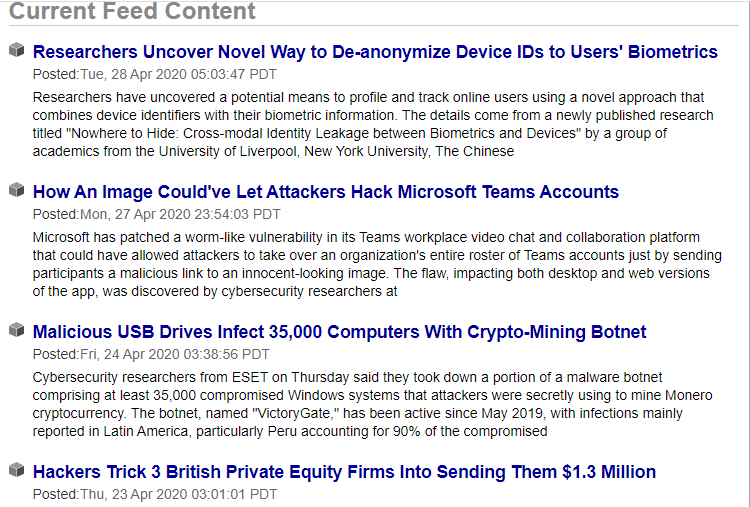
\includegraphics[scale=0.45]{Figures/cyber-feed}}
    \caption{Raw Cyber newsfeed from source \citep{news-feed}}
    \label{fig:cyber-feed}
\end{figure}
\FloatBarrier

Here, we see how a cyber newsfeed reading pane normally looks. 
It is a list of  cyber newsfeed items presented at a cyber news publishing  website \citep{news-feed}. 
The general construct of a cyber newsfeed item is 
1) one liner headline 
2) date and time of the cyber news posted and 
3) a more detailed paragraph about that particular news shown under the headline. 

The actual content of the detailed newsfeed item could be more, may be it is hosted with some pictures or links explaining some cyber issues and more detail on the particular cyber newsfeed item. Let see the other informations available in a cyber newsfeed item with an example from \citep{news-feed}.

For instance, the cyber news about \enquote{Malicious USB Drives…}, as shown in FIGURE \ref{fig:cyber-feed}, when accessed at \citep{news-feed} on the web-page gave more information about the cyber newsfeed item.  The extra information retrieved on the news item are the following: 

\begin{itemize}
  \item \textbf{Author} of this cyber newsfeed item.
  \item \textbf{Place of origin} of this cyber newsfeed item.
  \item \textbf{Impacted}  users, machines and servers.
  \item Potential \textbf{loss} due to Malicious USB Drives.
  \item \textbf{Mitigation} ways to avoid this.
\end{itemize}

The goal of a cyber newsfeed is to provide enough information about the cyber news topic at the time of the publication at the website. 
It is also good to know that publications of such cyber newsfeed items do not follow a common standard and the structure of the contents published vary from one website to another website. This was confirmed after comparing the contents of two websites\footnote{Look at Appendix \ref{AppendixChapter3} for the difference between \url{https://www.databreaches.net}
(figure \ref{fig:databreaches}) 
and content of 
\url{https://www.darkreading.com.} 
(figure \ref{fig:darkreading})} 
1) \url{https://www.databreaches.net} and 
2) \url{ https://www.darkreading.com}.

\section{Why do we need cyber newsfeed?}

The objectives of the cyber newsfeeds are to provide timely cyber awareness and information about  any ongoing cyber threats. With such informations, the organizations can prepare themselves to avoid or mitigate certain cyber risks which may impact business operations \citep{ring2014threat}. 
Such cyber informations acknowledged by the organisation  will ensure that the organization’s critical business information is safe from the vulnerabilities related to similar threats.
It helps organizations to understand the motivation of a threat actor\footnote{\url{https://en.wikipedia.org/wiki/Threat_actor}}, 
their behaviour and technique of attack \citep{jouini2014classification}. 
It also helps to identify the vulnerable system and the input points of attack. 
The designated and responsible cyber security team can use this information as a heads up and start analysing their situation and get prepare in case of a potential attack \citep{chismon2015threat}. 

Some examples of such information extracted from a cyber newsfeed items which may be useful for the awareness of security professionals, are as listed below:
\begin{itemize}
    \item \textbf{Indicators of Compromise (IOCs):} 
    System artefacts or observable that contain patterns, 
    such as malicious Internet Protocol addresses (IPs) or hashes of files containing malware, 
    which can help identify suspicious or malicious activity \citep{hyeisuncyber}.
    
    \item \textbf{Tactics, Techniques and Procedures (TTPs): }
    Description of the behaviour of an actor that can assist operational activities, such as details of exploits and malware delivery mechanisms. TTPs include tradecrafts, i.e., behaviour used to conduct a malicious activity, infrastructure used to deliver malicious content or maintain command and control capabilities, and attackers’ intentions 
    \citep{shahi2018tactics}. 
    
    \item \textbf{Security alerts:} 
    Notification, usually human-readable regarding security issues, such as vulnerabilities 
    \citep[page 189]{RFC2828}. 
    
    \item \textbf{Threat intelligence reports:} 
    Collections of threat intelligence for various topics, such as threat actors, malware and attack techniques 
    \citep{ring2014threat}. 
   
    
    \item \textbf{Vulnerabilities:} 
    Known weaknesses in software implementations or procedures, and corresponding mitigations, such as security patches. Although in the information security literature, vulnerabilities are not threats, they are considered as an important component in the cyber threat information sharing ecosystem 
    \citep{rantos2020interoperability}. 
    
\end{itemize}

\subsection{Practical usage in Security Operations Center
(SOC) department }

The security operations centre of any organization using Information Technology systems protects Information and Information systems, by performing tasks, like cyber Intel collection, analysis, distribution, creation and fusion
\citep{onwubiko2015cyber}. 
These cyber newsfeeds are also used in threat assessment and to establish new trend on old cyber newsfeeds items 
\citep{zimmerman2014ten}.

\subsection{Where does it fit into big picture?}

Since the cyber newsfeed items is a information and is related to Cyber, 
we can say that cyber newsfeed item is a kind of cyber information. 
I would say they are fuel to cyber threat
\citep[page 169]{RFC2828} Intelligence Sharing Platforms.  
In FIGURE \ref{fig:TIP-model}, 
the data as cyber newsfeed is being collected from various sources and 
is getting processed for a more actionable information transformation.

\begin{figure}
\centering
    \fbox{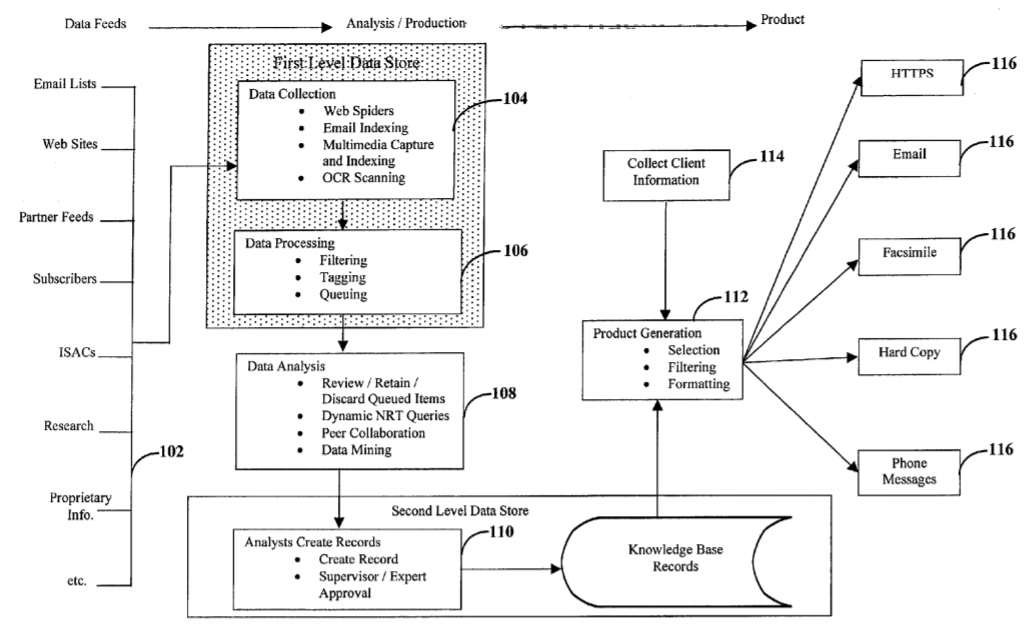
\includegraphics[scale=.63]{Figures/TIP-model.png}}
    \caption{System and Method of data collection, Processing, Analysis, and annotating Cyber threats \citep{edwards2002system}}
    \label{fig:TIP-model}
\end{figure}

\section{How are cyber newsfeeds made? Who are the producers?}

Cyber newfeed creation is a work of cyber security professionals working individually or for the organizations. 
These security professionals are the one, 
who focus on one or more security domains or practice and also keep learning from the hackers community 
\citep{mahmood2010moving}. 
They, then collaborate and share their respective findings about a certain threat or group of threats openly; 
among themselves, 
and on the internet as an information
or an intelligence for the awareness among security defenders. 
The focus area of such information may vary from vulnerabilities,
incident response, identifying intrusions, 
data breaches and potential threats 
\citep{rantos2020interoperability}. 
Vendors providing hardware and software products, 
manufactures of IT hardware and 
software products are also the major contributors of cyber newsfeed. 
For example, Microsoft releases information about its patches on its website\footnote{Microsft patches updates: \url{https://portal.msrc.microsoft.com/en-us/security-guidance.}}.

\section{How are cyber newsfeeds consumed? Who are the consumers?}

The collection and processing of cyber newsfeed  
depends on the purpose of cyber newsfeeds items. 
If the sole purpose is just reading then, 
an individual can explore the website producing cyber newsfeeds items 
his particular interests area.  
I want to highlight that, 
an automated collection system can also be configured 
to collect cyber newsfeed items from different sources and 
store in a single database 
\citep{sauerwein2017threat}. 
Another case is where specialized cyber security companies scan 
the web for all known and trusted cyber newsfeed and 
collect via dedicated servers into their own cyber Intelligence system 
to run analytics and make it selective and relevant. 
Like ON2IT has its own setup for collecting cyber newsfeed items. 
Cyber newsfeed consumers vary from people to organization, 
people may include security analysts, security officers, 
security advisors, security architects and general IT users 
\citep{shackleford2015s}.

\section{What are the sources of cyber newsfeeds?}

There is no “standard” list of 
cyber newsfeed or cyber information sources, 
however there are huge numbers of sources that are free and 
are open to access the cyber newsfeeds items. 
For illustration, 
here is a list of links that I have found as a good example on internet. 
The sources were working perfectly at the time of writing (Aug 2020) this thesis.
it is possible that some of the websites 
may not work at later point of time, 
but it is easy to find alternative websites containing similar information. 
The examples of the cyber newsfeed sources 
are based on different type of cyber newsfeed 
or information contents.

\begin{itemize}
    \item \textbf{General technology and security trends:} 
        \begin{itemize}
            \item Schneier on Security Blog: 
            \url{http://www.schneier.com} 
            
            \item Krebs on Security: 
            \url{http://krebsonsecurity.com}
            
            \item Security Dark Reading: 
            \url{http://www.darkreading.com}
            
            \item Slashdot: 
            \url{http://slashdot.org}
            
            \item Securosis: 
            \url{https://securosis.com/blog}
            
        \end{itemize}

    \item \textbf{Threat intelligence }
        \begin{itemize}
            \item Team Cymru (also has subscription service): 
            \url{http://www.team-cymru.org}
            
            \item FBI cybercrime information: 
            \url{http://www.fbi.gov/about-us/investigate/cyber/cyber}
            
        \end{itemize}
        
    \item \textbf{Malware and threats }
        \begin{itemize}
            \item SANS Internet Storm Center: 
            \url{http://isc.sans.edu}
            
            \item Dshield: 
            \url{http://www.dshield.org}
            
            \item Offensive Security’s Exploit Database: \url{http://www.exploit-db.com} 
            
        \end{itemize}
    
    \item \textbf{Bad domains, IP addresses, and other indicators} 
        \begin{itemize}
            \item Malware Domain List: 
            \url{http://www.malwaredomainlist.com}
            
            \item Unspam Technologies Project Honeypot: 
            \url{http://www.projecthoneypot.org/index.php}
            
            \item Shadowserver Foundation: 
            \url {http://www.shadowserver.org/wiki} 
            
        \end{itemize}
        
    \item \textbf{Automatic threat analyzers }
        \begin{itemize}
            \item Virustotal: 
            \url{http://www.virustotal.com}
            
            \item Metascan online: 
            \url{http://www.metascan-online.com}
            
        \end{itemize}
        
    \item \textbf{Patches and vulnerabilities} 
            \begin{itemize}
            \item MITRE’s\footnote{\url{https://en.wikipedia.org/wiki/Mitre_Corporation}} CVE: 
            \url{https://cve.mitre.org}
            
            \item NIST’s\footnote{\url{https://en.wikipedia.org/wiki/National_Institute_of_Standards_and_Technology}} National Vulnerability Database: 
            \url{http://nvd.nist.gov}
        \end{itemize}
        
\end{itemize}

Apart from these sources, 
some social networking sites like Twitter\footnote{Twitter link  \url{https://twitter.com/cyber}}
is also a very good source of sharing cyber related news 
and those can also be considered as cyber newsfeed.

\section{Keywords and definition}

\subsection{Artefact}	

Artefacts could be constructs, models, methods, 
and instantiations. 
They are built to address to unsolved problems 
\citep{march1995design}. 
Artefacts are output of design science research,
commonly used within Information technology to develop 
IT systems and related processes.

\subsection{Threat}	

A potential for violation of security, 
which exists when there is a circumstance, 
capability, action, or event 
that could breach security and cause harm.
That is, 
a threat is a possible danger that might exploit a vulnerability. 
A threat can be either "intentional" 
(i.e., intelligent; 
e.g., an individual cracker or a criminal organization) 
or "accidental" 
(e.g., the possibility of a computer malfunctioning, 
or the possibility of an "act of God" such as an earthquake, 
a fire, or a tornado) \citep[page 169]{RFC2828}.

\subsection{Attack}	

An assault on system security that derives from an intelligent threat, 
i.e., an intelligent act that is a deliberate attempt 
(especially in the sense of a method or technique) 
to evade security services and 
violate the security policy of a system 
\citep[page 13]{RFC2828}.

\subsection{Data Sources}	

An online source of cyber information owned and 
maintained by the owner of the website 
used to publish and share cyber information 
to cyber world 
\citep{eu2014cyber}. 
The sources could be with paid or free subscriptions.

\subsection{Feed}

A feed is a cyber information 
available at any cyber data source 
or cyber information source 
\citep{eu2014cyber}. 

\subsection{Vulnerability}	

A flaw or weakness in a system's design, implementation, 
or operation and management 
that could be exploited to violate the system's security policy
\citep[page 189]{RFC2828}.

\subsection{Computer emergency response team (CERT)}

An organization that studies computer and 
network INFOSEC in order to provide incident response services 
to victims of attacks, 
publish alerts concerning vulnerabilities and threats, 
and offer other information to help improve computer and network security
\citep[page 41]{RFC2828}.

\subsection{Digital Assets}

A digital asset is any text or media 
that is formatted into a binary source 
and includes the right to use it 
\citep{toygar2013new}.

\subsection{Threat Information}	

Cyber-threat information is any information 
that can help an organization to identify, assess, monitor,
and respond to cyber-threats. 
Examples of cyber-threat information include indicators 
(system artefacts
or observables associated with an attack), 
TTPs, security alerts, threat intelligence reports, 
and
recommended security tool configurations 
\citep{johnson2017cyber}.

\subsection{Threat intelligence:}	

Cyber threat intelligence is the task of 
converting cyber information 
into actionable insights 
by collecting evidence-based knowledge 
and evaluated in the context of reliability. 
Threat intelligence is used by organisational governance 
and management entities 
to protect digital assets 
and business information. 
This includes context, mechanisms, indicators, implications 
and actionable advice, 
about an existing or emerging cyber threats. 
The relevant cyber threat intelligence 
can be used to calculate risk 
and perform decisions to protect the digital assets including IT systems and business information. 
In the context of this paper 
it is important to make a note 
that cyber newsfeed mentioned in 
FIGURE \ref{fig:cyber-feed} 
is also a cyber information 
\citep{mavroeidis2017cyber}.



\subsection{Threat intelligence  platform}	

Threat Intelligence  Platform  
%\citep{wiki:TIP,dandurand2013towards} 
 Threat Intelligence Sharing Platform (TISP) can manage cyber threat intelligence data and convert this data into actionable intelligence, delivered to the different tools and assist in incident response has been introduced. Information security vendors and community are currently offering TISP solutions to provide threat intelligence feed and system that can assist cyber threat response. The solution can be divided into two categories which is content aggregation that can provide various threat data feeds and Threat Intelligence Management System for deriving business value from the collected information.
\citep{abu2018cyber}
\subsection{Collector or Data Collection engine}	



Data and Information 
is used interchangeably 
in this paper and data collection engine is a software that pushes new cyber intel  data into the system from a multitude of data sources like NIST’s National Vulnerability Database, Twitter, Reddit, Security blogs, dark web markets [9], etc.  The data is then stored in a database \citep{mittal2019cyber}.

%and data collector 
%is an essential functionality 
%of a Threat intelligence platform
%\citep{wiki:TIP} to collect cyber information 
%from multiple data sources.

\subsection{Processor}	

A term used to denote an engine or module 
which has key responsibilities 
of processing activities like filtration
\citep{CanAtasoy2019} 
of required data or information, 
tagging (enrichment) and context determination (contextualization)
within a Threat intelligence platform
\citep{CanAtasoy2019}.

\subsection{Analyser}

A term used to denote a engine or module 
which has key responsibilities of 
Analytics
activities  
\citep{CanAtasoy2019} 
like correlation within existing data or information, 
pattern discovery 
and other analytical capabilities within a Threat intelligence platform
\citep{CanAtasoy2019}.

\subsection{Publisher}	

A term coined to denote an engine or module 
for the artefact 
having capabilities of editorial tasks and delivery 
of the Cyber newsfeeds to the end users.

\subsection{IT Governance}	

IT governance is the responsibility of 
the Board of Directors and executive management.
It is an integral part of enterprise governance and
consists of the leadership and organizational
structures and processes that ensure that the
organization’s IT sustains and extends the
organization’s strategy and objectives 
\citep{guldentops2009board}.

\subsection{Information Security Management}	

A process of managing and safeguarding information 
and related systems 
in order to secure business information 
and digital assets
\citep{humphreys2016implementing}.

\subsection{IT System development}	

Development of a software based application for automation, 
compute or information sharing.

\section{Conclusion }
The terminologies and related concepts
described in chapter \ref{Chapter3key_concepts-and-terms} 
will be used in the further chapters
of this thesis.

